%-------------------------------------------------------------
\documentclass{beamer}
\usepackage[utf8]{inputenc}
\usepackage{hyperref}
\usepackage[T1]{fontenc}
\usepackage{tikz}

\usepackage{latexsym,xcolor,multicol,booktabs,calligra}
\usepackage{amsmath,amssymb,BOONDOX-cal,bm}	
\usepackage{graphicx,pstricks,stackengine}      
\usepackage{physics}
\usepackage{hyperref}
\usepackage{xcolor}
\usepackage{amsmath}
\usepackage{bm}
\usepackage{mathtools}

\author{}
%\titlegraphic{\includegraphics[width=\textwidth]{unilogo4cmittel.jpg}}
%\titlegraphic{ 
%\begin{tikzpicture}[overlay,remember picture]
%\node[right=-0.15cm] at (current page.150){
  %  \includegraphics[width=1.2\textwidth]{unilo%go4c.jpg}
%};
%\end{tikzpicture}
%}
\title{Blood Flow: Bridging the Micro-Macro Gap Using Scientific Machine Learning}
\institute{} 

%\logo{
\includegraphics[width=0.12\textwidth]{logo.png}}

\usepackage{Wue}

\def\cmd#1{\texttt{\color{red}\footnotesize $\backslash$#1}}
\def\env#1{\texttt{\color{blue}\footnotesize #1}}

\newtheorem{thm}{Theorem}[theorem]


%—-------------------------------------------------------------

\begin{document}
	\begin{frame}
    \titlepage
    \end{frame}

	
	\begin{frame}
		\tableofcontents[sectionstyle=show,subsectionstyle=show/shaded/hide,subsubsectionstyle=show/shaded/hide]
	\end{frame}
		
	
	%—------------------------------------------------------

	
	%-------------------------------------------------------	
	\section[Blood properties]{Familiarization with properties and modeling of Blood Flow}
	   % \subsection{}
		    \begin{frame}
			    \begin{itemize}
			    \item Blood consist of a suspension of elastic particulate cells:
\begin{itemize}
    \item \textbf{Red blood cells} ($\approx$ 40-45 \% of blood volume)
    \item White blood cells
    \item Platelets
\end{itemize}
in a liquid known as plasma ($\approx$ 55\% of blood volume)
			    \item Properties of Blood e.g. viscosity depend on physiological flow conditions, blood composition properties e.g. hematocrit, temperature, shear rate, cell aggregation, cell shape, cell deformation, orientation ...
			    			    \end{itemize}	
		    \end{frame}
		    
		 
	\begin{frame}
    	\begin{itemize}
    	\item While plasma has nearly Newtonian behaviour, whole blood exhibits non-Newtonian characteristics, particulary at low shear rates
    	\item   The Non-Newtonian characteristics of blood are:
			    \begin{enumerate}
			    \item Shear thinning
			    \item Yield stress (viscoplasticity)
			    \item Viscoelastic properties
			     \item Thixotropic behaviour
			    \end{enumerate}	
    	\end{itemize}
    \end{frame}
	
	
			    \begin{frame}
			    \begin{itemize}
			      	\item Non-Newtonian characteristics occur due to: \begin{itemize}
    	    \item Aggregation of RBC's at low shear rates (Rouleaux formation)
    	    \item Thixotropic behaviour due to finite time needed for RBC aggregation and disaggregation.
    	    \item Deformability of RBC and their tendency to align with flow field at high shear rates
    	\end{itemize}
    	\end{itemize}
			            \begin{table}[h]
    		\centering
    		\begin{tabular}{p{5cm}p{5cm}}
    			Low shear rates $\approx \hspace{5pt}< 1 \frac{1}{s}$ & High shear rates $\approx\hspace{5pt} > 400 \frac{1}{s}$ \\
    			\hline
    			apparent viscosity increases & apparent viscosity decreases \\
    		 yield stress & RBC's rotate \& accomadate flow\\
    		thixotropic  & \\
    	 RBCs aggregate are solid-like bodies, and  has ability to store elastic energy (viscoelastic) & RBCs behave fluid-like  bodies\\ 
    		\end{tabular}
    	\end{table}
		    \end{frame}
	%-----------------------------------------------------
	\section[Classical Mechanics]{Derivation of Navier-Stokes Equation from classical mechanics}
	    %\subsection{}

	
    \begin{frame}
    	\begin{figure}[thpb]
					\centering
					\resizebox{1\linewidth}{!}{
						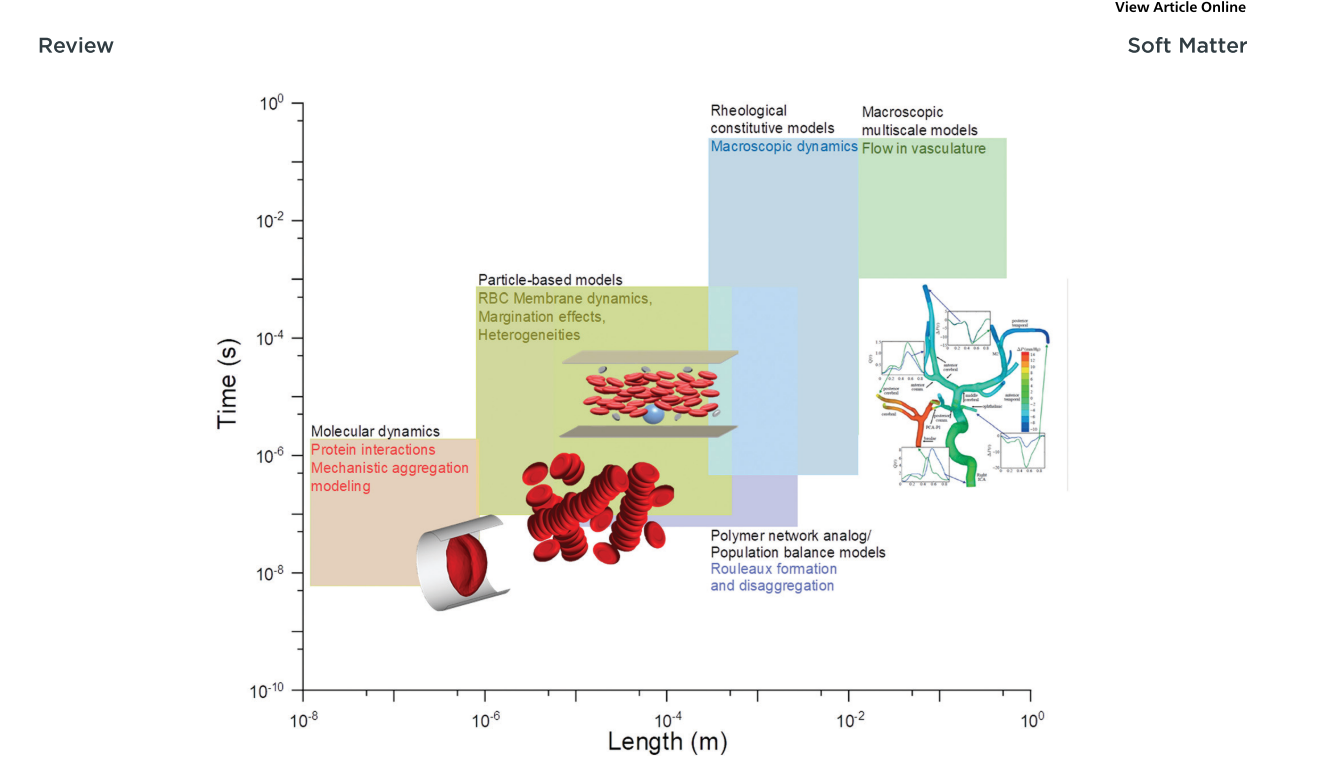
\includegraphics{models.png}
					}
					%	\includegraphics[scale=1.0]{figurefile}
					\caption{Length and time scales involved in blood flow modeling}
					\label{fig:1}
				\end{figure}
	    \begin{exampleblock}{} 
    		\begin{equation*}
    		f(x)=ax+b 
    		\label{eq1}
    		\end{equation*}
    	\end{exampleblock}
	
    	\begin{exampleblock}{\footnote{\tiny Test123}}
    		\begin{align}
    		    \vec{x}
    		    \begin{cases}
    			1 & 2\\
    			0 & 3\\
    		    \end{cases}
    	    	\label{eq2}
    		\end{align}
    	\end{exampleblock}
    \end{frame}
	
	
	    \begin{frame}
	    \begin{itemize}
	        \item        Classical Mechanics
			    $\Rightarrow$ Continuum hypothesis!
			    \item Starting point are mass and momentum conservation for incompressible fluids ($\rho \approx \text{const}$) and a constitutive equation, which describes material behaviour 
	    \begin{enumerate}
			    \item \begin{equation*}
			         \nabla \cdot \bm{u} = 0
			    \end{equation*}
			      \item \begin{equation*}
			         \rho  \frac{\partial \bm{u}}{\partial t} + \rho (\bm{u} \cdot \nabla) \bm{u} =  \nabla \cdot \bm{\sigma} + \rho\bm{f}
			    \end{equation*}
			    \item \begin{equation*}\bm{\sigma} = \underbrace{-p\bm{I} }_{\text{volumetric stress tensor}} + \underbrace{\bm{\tau}   }_{\text{deviatoric stress tensor}} \end{equation*}
			    \end{enumerate}	
			 
			    \item Newtonian assumption i.e. $
    \bm{\sigma} = \bm{\sigma}(\grad\bm{u},p)= -p\bm{I} +2\eta\bm{D}(\grad\bm{u})= -p\bm{I} + \eta(\grad\bm{u}+\grad\bm{u}^T)$
    with $\eta = \text{const}$ leads to well-known Navier-Stokes Equation
	    \end{itemize}
		    \end{frame}

	
	    \begin{frame}
	    \begin{itemize}
        \item Newtonian behaviour is a limitation usually accepted for blood flow in large arteries
        \item Non-Newtonian
characteristics $\Rightarrow$ In small size vessels or in regions of stable recirculation, (e.g. venous system) and parts of  arterial vasculature where geometry has been altered and RBC aggregates become more stable,
like downstream a stenosis or inside a saccular aneurysm
	    \end{itemize}
		    \end{frame}
	
	%-------------------------------------------------
	\section[Non-Newtonian Models]{Rheological Non-Newtonian models for blood}	
	
%	\begin{frame}<1->
%		 \begin{thm}
%	        contents...
%	        \label{thm-1}
%		 \end{thm}
%		\begin{block}{Test}<2->
%            This is a theorem.
 %           \begin{equation}
%                a^2 + b^2 = c^2
%            	\notag	
 %           	\label{equ-3}
 %           	\end{equation}
%        \end{block}
%    	
%		\begin{proof}<3->
  %          \textit{Trivial.} 
 %       \end{proof}
		            
  %      \begin{corollary}<4->
  %          This is a corollay.
    %        \begin{equation}
 %               c^2 = b^2 + a^2
  %              \label{equ-4}
  %          \end{equation}
   %     \end{corollary}
%	\end{frame}
	
	\begin{frame}%{Test}
		\begin{itemize}
			\item In order to account for Non-Newtonian effects, we can
			\begin{enumerate}
				\item use \textbf{time-independent constitutive equation} to close system and make the viscosity dependent of the
deformation rate tensor 
				\item use a (nonlinear) \textbf{viscoelastic constitutive equation} $\Rightarrow$ more complex constitutive equations
must be solved simultaneously along with the equations of conservation of mass and momentum (time dependent models)
\end{enumerate}
		\end{itemize}
		
		
		
	\end{frame}
	
	
		\begin{frame}{time-independent constitutive equation }
		\begin{itemize}
			\item Express the viscosity
as function of the strain rate $\Rightarrow$ Generalised Newtonian Model 
			\begin{equation}
			    \bm{\sigma} = \bm{\sigma}(\grad\bm{u},p)= -p\bm{I} +2\eta(\Dot{\gamma})\hspace{5pt} \bm{D}(\grad\bm{u})
			\end{equation}
			\item Examples are e.g. Power law model $\eta= k\Dot{\gamma}^{n-1}$, Extension of the power-law model from Walburn and Schneck (considered the dependence of $\eta$
on the haematocrit and total protein minus albumin content), Cassons equation (account for yield stress)  ...
			\item Computationally inexpensive to implement but cannot predict accurately
transient changes which are relevant as blood flows naturally under pulsatile conditions $\Rightarrow
$ viscoelastic model
		\end{itemize}
		
	\end{frame}

	\begin{frame}{Viscoelastic constitutive equation (time-dependent)}
		\begin{itemize}
		\item Split stress tensor approach: Decompose total stress tensor into its non-Newtonian (RBC influence) and Newtonian (plasma) parts 
			\item Different models (Maxwell model, Oldroyd-B model ...) considering e.g. viscoelasticity, viscoelasticity + yield stress, thixotropic elasto-visco-plastic behavior of blood ...
			\item We get additional equations (e.g. ODE's) to solve for
		\end{itemize}
		
	\end{frame}
	
	
	
	
	
	
	\begin{frame}{Questions}
		\begin{itemize}
		\item Do we want to examine a specific phenomena (e.g aneurysma) s.t. we can
focus from the variety of non-newtonian models (including shear thinning, plasticity, viscoelasticity, thixotropy, all together, etc.) on a specific group
\begin{itemize}
    \item What is the relevant diamter which we want to examine?
    \item What are our regions of interest?
    \item Heat transfer?
    \item I will neglect biochemical processes?
    \item FSI?
\end{itemize}
		\end{itemize}
		
	\end{frame}
	
	
	
	
	%----------------------------------------------
%	\section{References}
%		
%		\begin{frame}[allowframebreaks]
%			\bibliographystyle{unsrt}
%			\bibliography{Bibliography.bib}	
%		\end{frame}
%%
	%-------------------------------------------
%	\begin{frame}
%		\begin{center}
%			{\Huge \emph {\textrm{Thank  ~you!}}}
%		\end{center}
%	\end{frame}

\end{document}